\documentclass{article}
\usepackage{tikz}
\usepackage{lscape}
\usepackage{amsmath}
\usetikzlibrary{positioning}
\title{\vspace{-2cm}The Future of Mendelian Randomization Studies}
\author{MR Data Challenge}
\date{}
\usepackage{geometry}
\geometry{letterpaper}
\begin{document}

\maketitle

\subsubsection*{Part 3: Long-term exposure to "A" in women}

\noindent For simplicity, only 2 time points are depicted in the following DAG. The data-generating model will include a total of 6 time points: ages 20 to 30; 30 to 40; 40 to 50; 50 to 60; 60 to 70; 70 to 80.
\vspace{0.5 cm}
\begin{figure}[!h]
\centering
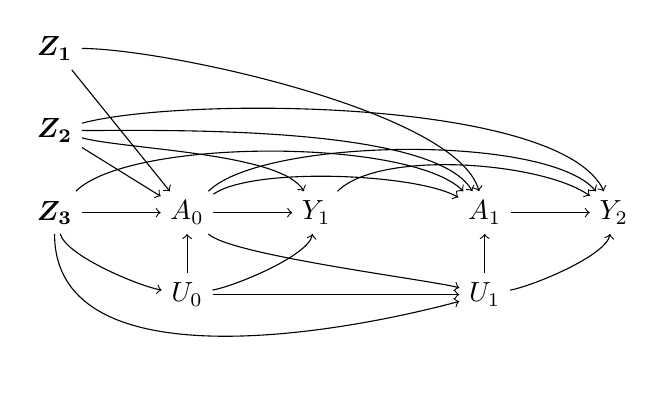
\begin{tikzpicture}
% Nodes at baseline %
\node[text centered, font=\boldmath] (z1) {{$Z_1$}};
\node[below=0.5 of z1, text centered, font=\boldmath] (z2) {$Z_2$};
\node[below=0.5 of z2, text centered, font=\boldmath] (z3) {$Z_3$};
\node[right=1 of z3, text centered] (a0) {$A_0$};
\node[below=0.5 of a0, text centered] (u0) {$U_0$};
\node[right=1 of a0, text centered] (y0) {$Y_1$};

% Nodes at time 1 %
\node[right=1.5 of y0, text centered] (a1) {$A_1$};
\node[below=0.5 of a1, text centered] (u1) {$U_1$};
\node[right=1 of a1, text centered] (y1) {$Y_2$};

% Edges %
\draw[->] (z1) -- (a0);
\draw[->] (z2) -- (a0);
\draw[->] (z3) -- (a0);
\draw[->] (z1) to [out=0, in=105, looseness=0.5] (a1);
\draw[->] (z2) to [out=0, in=120, looseness=0.5] (a1);
\draw[->] (z3) to [out=45, in=135, looseness=0.5] (a1);

\draw[->] (u0) -- (a0);
\draw[->] (u0) -- (u1);
\draw[->] (u1) -- (a1);
\draw[->] (u0) to [out=10, in=-100, looseness=0.5] (y0);
\draw[->] (u1) to [out=10, in=-100, looseness=0.5] (y1);

\draw[->] (a0) -- (y0);
\draw[->] (a1) -- (y1);
\draw[->] (a0) to [out=35, in=150, looseness=0.5] (a1);
\draw[->] (a0) to [out=45, in=130, looseness=0.5] (y1);

\draw[->] (a0) to [out=-45, in=165, looseness=0.3] (u1);

\draw[->] (y0) to [out=45, in=145, looseness=0.6] (y1);

\draw[->] (z2) to [out=-15, in=120, looseness=0.5] (y0);
\draw[->] (z2) to [out=15, in=115, looseness=0.5] (y1);

\draw[->] (z3) to [out=-75, in=170, looseness=0.5] (u0);
\draw[->] (z3) to [out=-90, in=195, looseness=0.9] (u1);

\end{tikzpicture}
\end{figure}

\noindent Note: {$\boldsymbol{Z_1}$} represents the set of SNPs located on chromosome 3 and 4; $\boldsymbol{Z_2}$ represents the set of SNPs located on chromosome 9; and $\boldsymbol{Z_3}$ represents the set of SNPs located on chromosome 17. Let $\boldsymbol{Z}=(\boldsymbol{Z_1}, \boldsymbol{Z_2}, \boldsymbol{Z_3})$.

\newpage
\noindent The data-generating model is as follows (note that data for $k=0$ and $k=1$ are generated in part 2):\\
$$
\begin{aligned}
k&=2,\dots,K \text{ where } K=5\\
%Z_{j,i}&\sim B(2, p_j) \text{ where } p_j\sim \mathcal{U}_{[0.1, 0.5]} \text{ for } 1\le j \le 11 \\
U_{k,i} &\sim \mathcal{N}\left(\boldsymbol{\beta_{ZU}^{'}Z_i} + \beta_{UU}U_{k-1,i} + {\beta_{AU}\frac{A_{k-1,i}-50}{10}}, \ 1 \right) \\
A_{k,i} &\sim \mathcal{N}\left(25+ \boldsymbol{(\beta_{ZA_{base}} + \beta_{ZA_\Delta}k)^{'}Z_i} + 
    \beta_{UA}U_{k,i} + \beta_{AA}^{'}A_{k-1,i}, \ 5 \right) \\
Y_{k+1,i} &\sim Bin\Bigg(1, \ \text{expit}\left(\log{\frac{\lambda}{1-\lambda}} + \boldsymbol{\beta_{ZY}^{'}Z_{i}} + 
    \beta_{UY}U_{k,i} +
    \beta_{AY_{k}}\frac{A_{k,i}-50}{10} +
    \beta_{AY_{k-1}}\beta_{AY_\Delta}\frac{A_{k-1,i}-50}{10}\right) \Bigg)\\ 
\end{aligned}
$$

\noindent where
$$
\begin{aligned}
\boldsymbol{\beta_{ZU}}&=(0, 0, 0, 0, 0, 0, 0, 0, 0.25, 0.10, 0.30)\\
\beta_{UU}&=0.50 \\
\beta_{AU}&=0.35 \\
\boldsymbol{\beta_{ZA_{base}}} &=(\beta_{ZA_{base,1}}, \beta_{ZA_{base,2}}, \dots, \beta_{ZA_{base,11}}) \text{ where } 
    \beta_{ZA_{base,j}}\sim\mathcal{U}_{[1,5]} \text{ for } 1\le j \le 11 \\
\boldsymbol{\beta_{ZA_\Delta}} &=(\beta_{ZA_{\Delta,1}}, \beta_{ZA_{\Delta,2}}, \dots, \beta_{ZA_{\Delta,11}}) \text{ where }
    \beta_{ZA_{\Delta,p}}\sim\mathcal{U}_{[-\frac{1}{k}\beta_{ZA_{base,p}}, \ \frac{1}{k}\beta_{ZA_{base,p}}]} \\ 
\beta_{UA}&=5 \\
\beta_{AA}&=0.5 \\
\boldsymbol{\beta_{ZY}} &=(0, 0, 0, 0.1, 0.05, 0.3, 0.2, 0.01, 0, 0, 0) \\
\beta_{UY}&=0.3  \\
\beta_{AY_{k}}&=\begin{cases}
    0.2 &\text{if } k=0 \\
    0.3 &\text{if } k=1 \\
    0.7 &\text{if } k=2 \\
    0.3 &\text{if } k=3 \\
    0.2 &\text{if } k=4 \\
    0.1 &\text{if } k=5 \\
\end{cases} \\
\beta_{AY_{\Delta}}&=0.5 \\
\end{aligned}
$$

\end{document}
